% Section 6 page 618
\documentclass{article}
% List all of the packages used in all of the files, which can the just be added as an input.
\usepackage[margin=1in]{geometry}
\usepackage{titlesec}
\usepackage{amsmath}
\usepackage{subfiles}
\usepackage{mathptmx}
\usepackage{csvsimple-l3}
\usepackage[T1]{fontenc}
\usepackage[utf8]{inputenc}
\usepackage{tabularx,ragged2e,booktabs,caption}
\usepackage{tikz}
\usepackage[colorlinks=true,allcolors=blue]{hyperref}
\usepackage{graphicx}
\usepackage{changepage}
\usepackage{natbib}
\usepackage{longtable}
\usepackage{abstract}
\usepackage{atbegshi}% http://ctan.org/pkg/atbegshi

\begin{document}
\section{ESTIMATION RESULTS AND SIMULATION EXPERIMENTS}
\label{section:estimation}
6.1.     \textit{Main Estimation Results.}    We report the parameter estimates in Table \ref{tab:EstimationResults}. The key result is the estimate of the disutility of labor parameter, which is 1.262. The implied elasticity of intertemporal substitution is
$$ i.e.s. \equiv b_2 \equiv \dfrac{1}{a_2-1} = 3.820 $$
\subfile{../Tables/Table4.tex}
This elasticity estimate is reasonably close to the elasticity parameter macroeconomists typically use to calibrate real business cycle models (e.g., \cite{Eichenbaum1988-kg}, obtain an elasticity estimate that is around 5, and \cite{Prescott1986-vn}, uses 2 in his calibration exercise). \par
Another key parameter of interest is $a_1$, the CRRA parameter, which we estimate to be 0.262. Thus, the intertemporal elasticity of substitution in consumption (i.e.s.-c) is
$$ \dfrac{1}{a_1-1} = -1.354$$
This is quite different from conventional estimates. Typically, $a_1$ is estimated to be around -2, which implies that the i.e.s.-c is around -1/3 (see \cite{Hubbard1994-qp}). \cite{Keane2001-yk} also estimate a dynamic model of labor supply, human capital accumulation, and saving, and they obtain an estimate of the i.e.s.-c, which is around -2 (i.e., $a_1 \approx 0.5$), which is more similar to our estimate of i.e.s.-c = -1.354 than most of the prior literature. \cite{Keane2001-yk} (p. 1078) argue that prior estimates of this i.e.s.-c had to imply a high degree of prudence (2 - $a_1$) in order to rationalize the fact that youths with steep age-earnings profiles do not borrow substantially against future income. They argue that their estimate of $a_1$ is larger than the values of about -2 typically estimated in the literature because their model incorporates borrowing constraints. Similarly, we use age effects in the marginal utility of consumption to help explain the failure of youths to borrow against future income. This may account for our larger estimate of $a_1$. Recently, \cite{Goeree2000-la} have argued that experimental evidence is consistent with $a_1 \approx 0.50$. \par
\hypertarget{HCprodfuncAgeWageProfiles}{}
\begin{figure}[tbp]
  \centerline{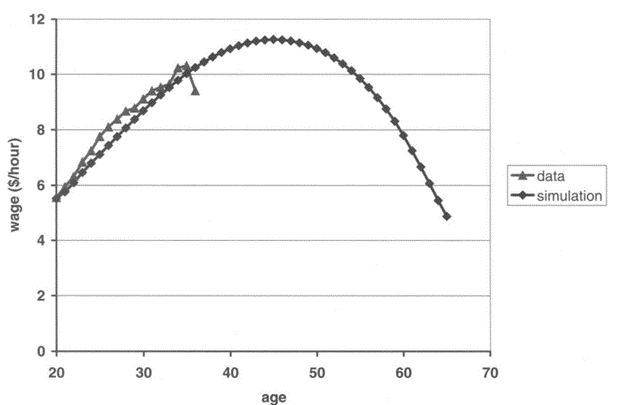
\includegraphics[width=6in]{../FigDir/Figure3.png}}
  \caption{AGE-WAGE PROFILES}
  \label{fig:AgeWageProfiles}
\end{figure}

\medskip
6.2.     \textit{Model Fit.}     To evaluate the fit of the model, we artificially generated 1000 individual life-cycle paths from ages 20 to 65 using the estimated parameters. The various age profiles in the simulated data are reported in Table \ref{tab:SimulatedProfiles}. Figures \ref{fig:AgeWageProfiles}-\ref{fig:AgeAssetProfiles} compare simulated age profiles of wages, labor supply, and assets with those of the data. The simulated profiles resemble the actual profiles reasonably well. Notice that the age-hours profile before retirement is rather flat compared to the significant humped shape of the simulated age-wage profile. The model is able to reconcile this fact with a large i.e.s. because of the human capital effect, as we have discussed earlier. \par
% Table 5
%\documentclass[10pt, letterpaper]{article}
%\usepackage{csvsimple-l3}
%\usepackage[T1]{fontenc}
%\usepackage[utf8]{inputenc}
%\usepackage{tabularx,ragged2e,booktabs,caption}
%\captionsetup[table]{labelsep=space}

%\begin{document}

\begin{center}
  \hypertarget{SimulatedProfiles}{}
  \begin{table}
  \centering
    \caption{ \label{tab:SimulatedProfiles}\\
      \scriptsize SIMULATED MEAN AGE PROFILES}
  \begin{tabular}{lllll}
    \hline%
    Age  & Mean Wage & Mean Hours & Mean Assets & $[(1+r) \beta]^{t-20} u_C(t)$ \\ \hline
20 & 5.517 & 1899.4 & 3239.2 & $1.26 \times 10^{-5}$ \\
21 & 5.754 & 1943.0 & 4031.4 & $1.27 \times 10^{-5}$ \\
22 & 6.088 & 1993.7 & 4614.1 & $1.26 \times 10^{-5} $\\
23 & 6.464 & 2040.5 & 5942.4 & $1.25 \times 10^{-5} $\\
24 & 6.799 & 2087.6 & 6784.4 & $1.24 \times 10^{-5} $\\
25 & 7.114 & 2132.9 & 7977.7 & $1.24 \times 10^{-5}$ \\
26 & 7.437 & 2176.8 & 9182.3 &$ 1.24 \times 10^{-5} $\\
27 & 7.754 & 2219.3 & 10,389 &$ 1.24 \times 10^{-5}$ \\
28 & 8.066 & 2260.5 & 11,582 & $1.24 \times 10^{-5}$ \\
29 & 8.378 & 2300.1 & 12,744 & $1.24 \times 10^{-5}$ \\
30 & 8.685 & 2337.3 & 13,842 &$ 1.24 \times 10^{-5} $\\
31 & 8.974 & 2372.9 & 14,834 & $1.24 \times 10^{-5}$ \\
32 & 9.256 & 2406.6 & 15,674 & $1.25 \times 10^{-5} $\\
33 & 9.526 & 2437.8 & 16,300 & $1.25 \times 10^{-5} $\\
34 & 9.784 & 2466.4 & 17,820 & $1.25 \times 10^{-5} $\\
35 & 10.03 & 2492.0 & 20,230 & $1.25 \times 10^{-5}$ \\
36 & 10.25 & 2515.1 & 23,517 & $1.25 \times 10^{-5} $\\
37 & 10.45 & 2534.7 & 27,656 & $1.25 \times 10^{-5} $\\
38 & 10.63 & 2551.0 & 32,615 & $1.25 \times 10^{-5} $\\
39 & 10.79 & 2562.3 & 38,344 & $1.25 \times 10^{-5} $\\
40 & 10.92 & 2569.5 & 44,772 & $1.25 \times 10^{-5}$ \\
41 & 11.04 & 2572.6 & 51,828 & $1.25 \times 10^{-5}$ \\
42 & 11.14 & 2569.8 & 59,432 & $1.25 \times 10^{-5} $\\
43 & 11.20 & 2560.2 & 67,494 & $1.25 \times 10^{-5} $\\
44 & 11.24 & 2545.0 & 75,890 & $1.25 \times 10^{-5} $\\
45 & 11.27 & 2522.1 & 84,519 & $1.25 \times 10^{-5} $\\
46 & 11.25 & 2491.4 & 93,256 & $1.25 \times 10^{-5} $\\
47 & 11.21 & 2452.0 & 101,973 & $1.25 \times 10^{-5} $\\
48 & 11.14 & 2402.2 & 110,531 & $1.25 \times 10^{-5} $\\
49 & 11.06 & 2342.0 & 118,779 & $1.25 \times 10^{-5} $\\
    50 & 10.94 & 2271.1 & 126,622 & $1.25 \times 10^{-5}$\\
51 & 10.79 & 2189.6 & 133,972 & $1.26 \times 10^{-5} $\\
52 & 10.60 & 2096.7 & 140,751 & $1.26 \times 10^{-5} $\\
53 & 10.38 & 1990.8 & 146,866 & $1.27 \times 10^{-5} $\\
54 & 10.13 & 1872.9 & 152,228 & $1.27 \times 10^{-5} $\\
55 & 9.849 & 1742.5 & 156,759 & $1.28 \times 10^{-5} $\\
56 & 9.530 & 1597.5 & 160,371 & $1.30 \times 10^{-5} $\\
57 & 9.161 & 1441.1 & 162,959 & $1.31 \times 10^{-5}$ \\
58 & 8.755 & 1274.1 & 164,440 & $1.32 \times 10^{-5} $\\
59 & 8.309 & 1102.0 & 164,709 & $1.33 \times 10^{-5} $\\
60 & 7.799 & 933.21 & 163,702 & $1.34 \times 10^{-5} $\\
61 & 7.250 & 777.70 & 161,383 & $1.35 \times 10^{-5}$ \\
62 & 6.669 & 633.47 & 157,795 &$ 1.36 \times 10^{-5}$ \\
63 & 6.070 & 488.99 & 153,096 & $1.38 \times 10^{-5}$ \\
64 & 5.452 & 434.42 & 147,231 & $1.45 \times 10^{-5}$ \\
65 & 4.877 & 251.58 & 141,247 & $1.36 \times 10^{-5}$ \\
    \hline
  \end{tabular}
  \end{table}
\end{center}

%\end{document}

\hypertarget{AgeHoursProfiles}{}
\begin{figure}[tbp]
  \centerline{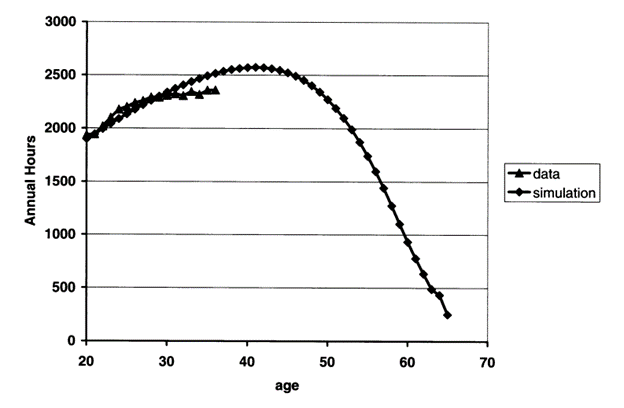
\includegraphics[width=6in]{\FigDir/Figure4}}
  \caption{AGE-HOURS PROFILES}
  \label{fig:AgeHoursProfiles}
\end{figure}

\hypertarget{AgeAssetProfiles}{}
\begin{figure}[tbp]
  \centerline{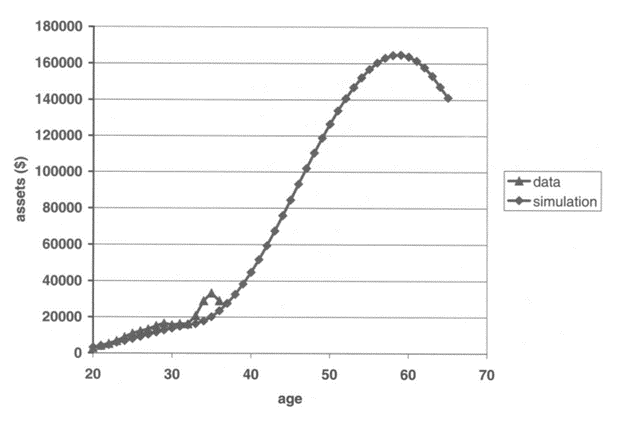
\includegraphics[width=6in]{../FigDir/Figure5.png}}
  \caption{AGE-ASSET PROFILES}
  \label{fig:AgeAssetProfiles}
\end{figure}

The simulated asset paths indicate that, even though labor income is small when people are young, individuals do not go into sizeable debt early in their life. In a model with perfect capital markets, this implies that, for the same consumption level, the value of consumption is smaller when people are young. As noted earlier, alternative explanations could be the existence of some finance constraints (see \cite{KeaneandWolpin2001}) or some nonseparability between consumption and labor. We did not pursue these explanations in this article. The out-of-sample predictions of the model for wages, hours, and assets look quite reasonable. The simulated age-hours path predicts retirement behavior of the agents at older ages, although that occurs somewhat sooner in the simulation than has been the case in the United States. On the other hand, later cohorts have been retiring at younger ages, so we cannot rule out that this prediction may be accurate for the cohort  used here. It is also worthwhile to notice that the model predicts large asset accumulation between ages 40 and 60, and dissaving afterwards, which is the actual pattern of savings and dissavings (see \cite{Carroll1996-yj}). \par
The performance of the approximate DP solution can be indirectly inferred from the age profile of the discounted marginal utility of consumption. In Table \ref{tab:SimulatedProfiles}, we report the simulated mean age profile of $[(1.0 + r)\beta]^{t-20} u_C(Ct, t)$, which should be constant over age.\footnote[11]{The model allows the value that agents place on consumption to vary with age, as determined by the $A(t)$ term in $U(c_t, t)$. According to our estimates, for a high school graduate, $A(t)$ is equal to $C_0$ times 0.524 (=$C_1$) at age 20, it rises to $C_0$ times 0.6913 (=$C_1 + C_2$) at age 25, and then rises to $C_0$ times 1.0 at age 33 and above. Results for other education categories are similar. Thus, at younger ages, less consumption is needed to reduce the marginal utility of consumption to any given level.} The profile is roughly constant, except it rises a bit in the late 50s and 60s. This gives indirect evidence that the solution algorithm seems to work fairly well overall. \par
\medskip
6.3.     \textit{Using Simulation Exercises to Assess the Bias in Conventional Elasticity Estimates.}     Using the simulated data, we conduct OLS and IV exercises to estimate the elasticity of intertemporal substitution using the methods of MaCurdy and Altonji. That is, we estimate the following equation via OLS and IV:
$$ \Delta \text{ln}(h_t) = \text{Const} + b_2 \Delta \text{ln}(W_t) + \zeta_t$$
where $\zeta_t$ is an error term. From the values of estimated coefficient $b_2$, we also recover the disutility of labor parameter as follows:
$$ a_2 = \dfrac{1}{b_2} + 1 $$
In Table \ref{tab:OLSIV}, we report the results of estimation on simulated data, and in Table \ref{tab:OLSIVClean}, we report the results of estimation on the simulated data that we cleaned by using an outlier elimination procedure that is similar to \cite{MaCurdy1981-iy}.\footnote[12]{The outlier elimination rules are:
  \begin{enumerate}
      \item Annual hours worked must be less than 4680 hours.
      \item For the calculation of changes in log earnings, the absolute value of the difference in a person's average hourly earnings in adjacent years cannot exceed \$16 or a change of 200\%.
        \item For the calculation of the changes in log hours, the absolute value of the difference in the annual hours of work in adjacent years cannot exceed 3000 hours or a change of 190\%.
        \end{enumerate}} The instruments for our IV exercise include a constant term, experience, experience squared, and the twice lagged wage. All the OLS and IV results are the average of 10 repetitions with independently simulated data. We used various age groups for the exercise, starting with simulation from age 20 to 64. Then, in Table \ref{tab:Altonji} we obtained results with ages from 20 to 56, 20 to 46, and 20 to 36, which is the age group in the NLSY79. \par
      % Table 6
%\documentclass[10pt, letterpaper]{article}
%\usepackage{csvsimple-l3}
%\usepackage[T1]{fontenc}
%\usepackage[utf8]{inputenc}
%\usepackage{tabularx,ragged2e,booktabs,caption}
%\captionsetup[table]{labelsep=space}

%\begin{document}

\begin{center}
  \hypertarget{OLSIV}{}
  \begin{table}
  \centering
    \caption{ \label{tab:OLSIV} \\
      \scriptsize ML, OLS, IV RESULTS}
    \begin{tabular}{llll}
\hline Age & & $b_2$ & $a_2$ \\
\hline $20-36$ & ML & $3.82(0.0124)$ & $1.26(0.000850)$ \\
\multicolumn{2}{l}{ Simulated data } & & \\
$20-64$ & OLS & $-0.444(0.00248)$ & $-1.25(0.0126)$ \\
& 3SLS & $0.971(0.0941)$ & $2.03(0.0999)$ \\
$20-56$ & OLS & $-0.301(0.00247)$ & $-2.33(0.0273)$ \\
& 3SLS & $1.13(0.259)$ & $1.89(0.204)$ \\
$20-46$ & OLS & $-0.270(0.00280)$ & $-2.70(0.0382)$ \\
& 3SLS & $0.537(0.217)$ & $2.86(0.753)$ \\
$20-36$ & OLS & $-0.293(0.00366)$ & $-2.41(0.0426)$ \\
& 3SLS & $0.325(0.256)$ & $4.08(2.42)$ \\
\multicolumn{2}{l}{ NLSY79 data } & & \\
$20-36$ & OLS & $-0.231(0.00659)$ & $-3.33(0.124)$ \\
& 3SLS & $0.260(0.0769)$ & $4.85(1.14)$ \\
      \hline
      \multicolumn{4}{l}{NOTE: Delta method is used to calculate the standard errors for $b_2$ for}\\
      \multicolumn{4}{l}{ML and $a_2$ for OLS and 3SLS results.}\\
      \multicolumn{4}{l}{Std. errors are in parentheses. Instruments: const, experience (which}\\
      \multicolumn{4}{l}{is age-19), experience squared, twice lagged wage.}\\
  \end{tabular}
  \end{table}
\end{center}

%\end{document}

      \hypertarget{OLSIVClean}{}
\begin{table}

  \centerline{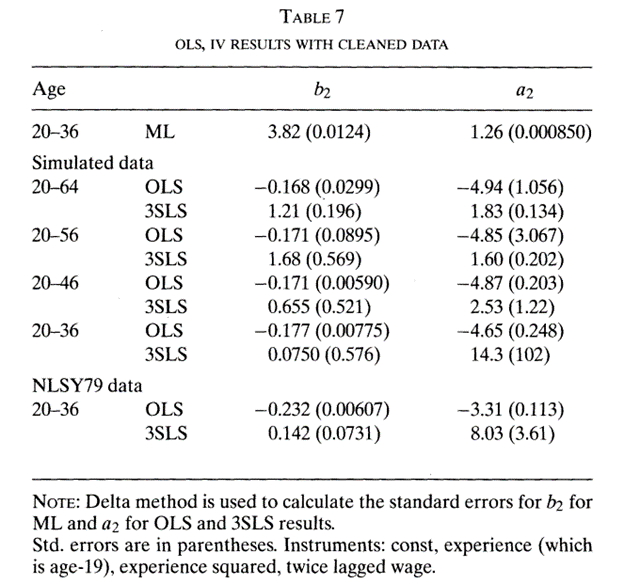
\includegraphics[width=4in]{\TablesDir/Table7.png}}
  \caption{\scriptsize OLS, IV RESULTS WITH CLEANED DATA} 
  \label{tab:OLSIVClean}
\end{table}
      Note that in Tables \ref{tab:OLSIV} and \ref{tab:OLSIVClean}, the elasticity estimates obtained from the simulated data using conventional methods are low, compared to the true value used to generate the data (3.820). This is true regardless of whether we remove outliers or not, which indicates that the downward bias does not depend much on the outliers. That is, the true i.e.s. in the simulated data is much higher than the estimates obtained using conventional IV methods. These results confirm the point that we get biased (toward 0) estimates of the i.e.s. if we do not explicitly allow for human capital accumulation in the model. \par
      \hypertarget{Altonji}{}
\begin{table}
  \centerline{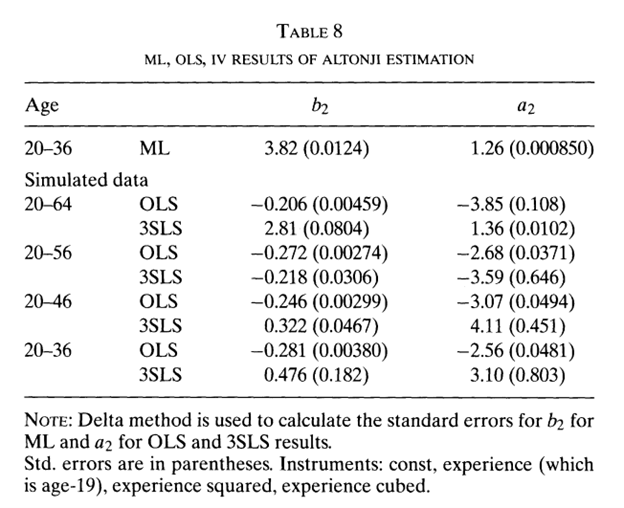
\includegraphics[width=6in]{\TablesDir/Table8.png}}
  \caption{\scriptsize ML, OLS, IV RESULTS OF ALTONJI ESTIMATION} 
  \label{tab:Altonji}
\end{table}
      Also note that the OLS estimates of the intertemporal elasticity $b_2$ are much smaller than the IV estimates. The theory implies that in the OLS case, there is another reason for downward bias because, in this case, the error term is correlated with the regressor due to the income effect. This is confirmed in our numerical example. \par
      It is also interesting to examine how the IV estimates vary with the age composition of the simulated data. It seems that if older individuals are heavily represented in the data, then the elasticity estimates tend to increase, with the maximum elasticity estimates being on average those obtained using the 20-56 age group. In particular, for that age group, we obtain 1.13 using the raw simulated data, and 1.68 using the simulated data without outliers. For younger age groups, the elasticity estimates are much lower, for example, for the 20-36 age group using all the simulated data, we obtain 0.325, which drops to 0.0750 when outliers are removed. Those results underscore the fact that the human capital component of the return to labor supply is much greater for the young. \par
      We also report (in the bottom panel of Tables \ref{tab:OLSIV} and \ref{tab:OLSIVClean}) the IV results obtained from the NLSY79 data that were used to obtain the ML estimates. The elasticity estimates are: 0.260 for the original NLSY79 data and 0.142 for the cleaned data. These estimates of the i.e.s. are much smaller than the one derived from the ML estimation, again suggesting that failure to account for human capital accumulation leads to downward bias.\par
\medskip
      6.4.     \textit{More on Model Fit.}     A comparison of OLS estimation results on the NLSY79 and on the simulated data is another method of assessing the fit of the model. Notice that for the age group 20-36, the OLS estimates of a regression of the log hours change on the log wage change produces similar results for the simulated and NLSY79 data. The OLS estimate from the simulated data is -0.293 whereas that from the NLSY79 data is -0.231 (see Table \ref{tab:OLSIV}, bottom 2 panels). Thus, the model seems to reproduce not only the average age profiles of the data, but also the negative raw correlation between log wage changes and log hours changes observed in the data. \par
      \hypertarget{Regressions1}{}
\begin{table}
  \centerline{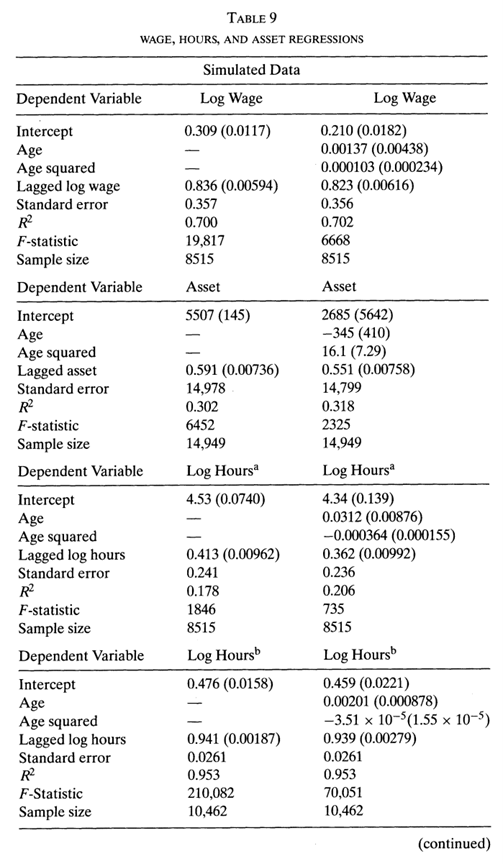
\includegraphics[width=6in]{\TablesDir/Table9pt1}}
  \caption{\scriptsize WAGE, HOURS, AND ASSET REGRESSIONS} 
  \label{tab:Regressions1}
\end{table}
      \hypertarget{Regressions2}{}
\begin{table}[tbp]
  \centerline{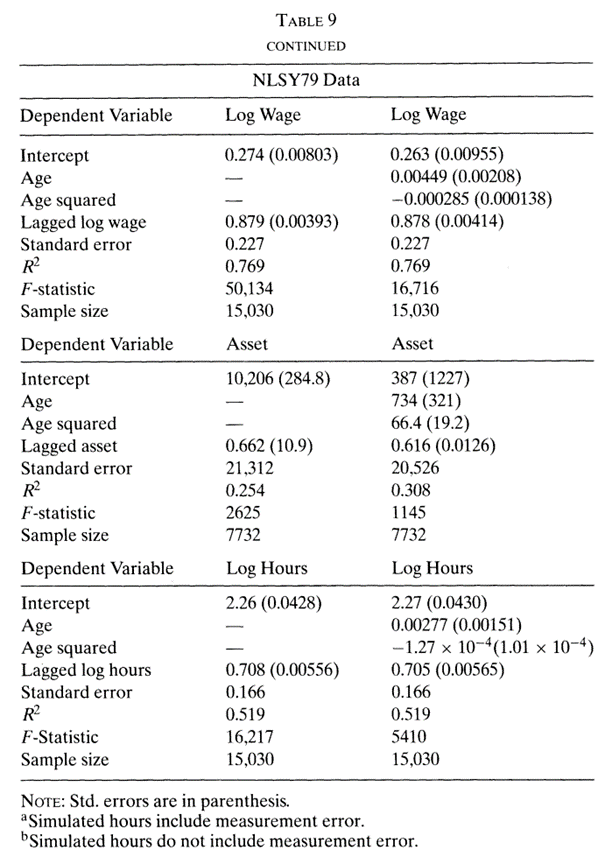
\includegraphics[width=6in]{../Tables/Table9pt2.png}}
  \caption{\scriptsize CONTINUED} 
  \label{tab:Regressions2}
\end{table}
      It is also interesting to compare the persistence of wages, hours, and assets in the simulated versus the actual data. In Table \ref{tab:Regressions1}, we report results where we regress the log wage, log hours, and assets from the simulated and NLSY79 data on a constant term, lagged values and age variables. For both the simulated and NLSY79 data, we removed outliers. The results show that the estimated model captures well the persistence of the log wages and assets in the data. For the regression using the simulated wage data, the coefficient of the lagged log wage is 0.836 if age variables are not included, and 0.823 if the age variables are included. In the regression using the NLSY79 data, these coefficients are 0.879 and 0.878, respectively. In the regression using simulated assets, the coefficient on lagged assets is 0.591 if the age variables are not included, and 0.551 if the age variables are included. In the regression using the NLSY79 data, these coefficients are 0.662 and 0.616, respectively. \par
      On the other hand, in the hours regressions, there are some discrepancies in the persistence coefficients between the simulated and NLSY79 data. For the  regression using simulated hours data, the persistence coefficients are 0.413 without age effects and 0.362 with the age effects. These coefficients are much lower than those using the NLSY data, i.e., 0.708 and 0.705, respectively. One potential reason for the discrepancy may be the assumption made in the model that the measurement error of hours is i.i.d. normally distributed, which may have been overly simplistic. In order to examine the effect of this assumption, we report results of another regression using the simulated data of log hours that does not include any measurement error. In this regression, the coefficient of the lagged log hours is 0.941 without age effects and 0.939 with age effects. These results imply that it is the measurement error that reduces the persistence of the simulated log hours in the original regression. An estimation exercise using a model that allows for a richer specification of measurement error is left for future research. \par
\medskip
      6.5.     \textit{How Human Capital Accumulation Affects Estimated and Actual Labor Supply Elasticities}     To assess the importance of human capital accumulation for the labor supply decision, we also report in Table \ref{tab:SimulatedMRS} the age profile of the mean marginal rate of substitution between consumption and labor supply, and the marginal rate of substitution divided by the wage. The latter is also shown in Figure \ref{fig:SimulatedMRS}. Note that the marginal rate of substitution is significantly higher than the real wage early in life. At age 20 it is 2.0 times greater than the real wage. Then, the marginal rate of substitution becomes closer to the actual wage rate at later stages of the career. The bias in the MaCurdy and Altonji estimation method arises from the fact that they do not recover the marginal rate of substitution, or the "effective wage," which is higher than the observed wage when there is human capital accumulation. \par
     \hypertarget{SimulatedMRS}{}
\begin{table}
  \centerline{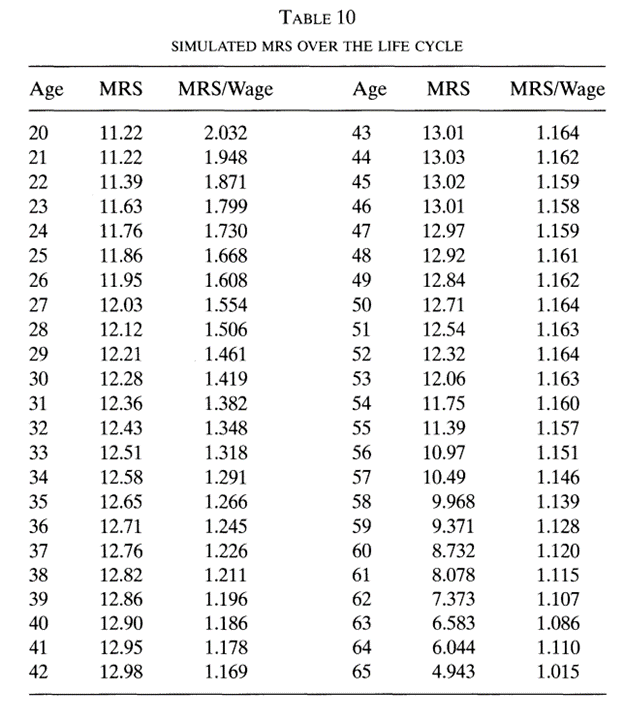
\includegraphics[width=6in]{\TablesDir/Table10}}
  \caption{\scriptsize SIMULATED MRS OVER THE LIFE CYCLE} 
  \label{tab:SimulatedMRS}
\end{table}
      \hypertarget{SimulatedMRS}{}
\begin{figure}[tbp]
  \centerline{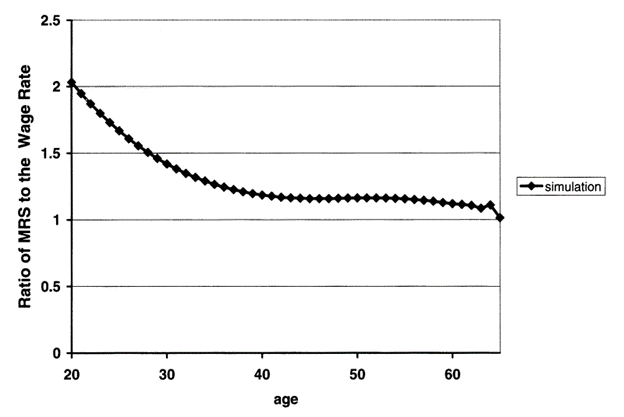
\includegraphics[width=6in]{../FigDir/Figure6.png}}
  \caption{SIMULATED MRS/WAGE PROFILES}
  \label{fig:SimulatedMRS}
\end{figure}

      This brings us to an important point, which is that IV methods cannot be used to solve the problem of bias in estimates of the substitution elasticity created by human capital accumulation. The reason that standard IV results are biased can best be described as follows. Define $W_t$ as the marginal rate of substitution between labor supply and consumption in period $t$. Also, define
      $$ \eta_t = \text{ln}(\tilde{W}_t) - \text{ln}(W_t) $$
    Then, from the definition of the marginal rate of substitution,
    $$  \text{ln}(\tilde{W}_t) =  \text{ln} b -  \text{ln} A(t) + (a_2 - 1)  \text{ln} h_t - (a_1 - 1)  \text{ln} C_t +  \text{ln} \epsilon_{2,t}$$
    If we first difference away the consumption term, we get the following expression:
    \begin{equation*}
      \begin{split}
        \Delta  \text{ln}(h_t) & = \text{Const} + \dfrac{1}{a_2 - 1} \Delta  \text{ln} (\tilde{W}_t) + \zeta_t \\
        & =  \text{Const} + \dfrac{1}{a_2 - 1} \Delta  \text{ln} (W_t) + \dfrac{1}{a_2 - 1} \Delta \eta_t + \zeta_t
           \end{split}
          \end{equation*}
        where $\zeta_t$ is a function of the error term $u_t$ in the log linearized consumption Euler equation and of $\Delta \text{ln} \epsilon_{2,t}$:
        $$ \zeta_t = -\dfrac{1}{a_2-1}(u_t + \Delta \text{ln} \epsilon_{2,t}.$$
        Note that, using equation \eqref{eq:FOC}, $\eta_t$ can be expressed as follows:
        $$ \eta_t = \text{ln} (\tilde{W}_t) -\text{ln} (W_t) \approx \text{ln} \dfrac{h_h \beta E \epsilon_{1,t+1} V_{K,t+1}}{u_C W_t}$$
        The problem is that conventional instruments for $\Delta \text{ln}(W_t)$ are correlated with $\Delta \eta_t$. For example, age is correlated with the expected marginal value of human capital, $E V_{K,t+1}$. The older the individual, the closer he is to the retirement period, hence the less the number of possible future periods where human capital is used. Therefore, the older the individual, the less the marginal value of human capital. Table \ref{tab:SimulatedMRS} shows how $\Delta \eta_t$ is negatively correlated with age, because the human capital effect decreases with age. In this case, the elasticity estimates from IV estimation using age as one of the instruments will likely be negatively biased. More generally, any variable that helps to predict wage growth ($\Delta \text{ln}(W_t)$) is likely to be correlated with $V_K (t + 1)$ and $U_C$. \par
        To further illustrate how conventional methods of estimation are biased, we also report the results based on the \cite{Altonji1986-zf} method of IV estimation, where consumption is used as a proxy for marginal utility of wealth. That is, we use the simulated data to estimate the equation
        $$ \text{ln}(h_t) = \text{Const} + \dfrac{1}{a_2 - 1} \text{ln}(W_t) + \dfrac{a_1 -1}{a_2 - 1} \text{ln} C_t - \dfrac{1}{a_2 - 1} \text{ln} \epsilon_{2,t}$$
        As we did not simulate measurement error in consumption, we used the simulated consumption value without measurement error as the regressor, together with simulated wage with measurement error. The intertemporal elasticity is again estimated to be much lower than the true value, confirming our claim that omission of human capital effects biases the elasticity estimates downwards. In Figure \ref{fig:AgeShadow}, we plot the age-wage profile, which corresponds to the substitution effect, or the marginal return to labor supply from increasing wage income (which, in this case, is the real wage). We also plot the age-human capital effect profile, which is the real value of the marginal return to labor supply from increasing human capital (which, in this case, is $\beta E_t g_h \epsilon_{1,t+1} V_{K, t+1}(A_{t+1}, K_{t+1}, \epsilon_{2,t+1})/u_C(C_t, t))$. We can see that until the age 50, the increase in substitution effect cancels out with the human capital effect, resulting in their sum (which is the total shadow value of labor supply) being roughly flat. As discussed earlier, this explains the flat age-hours profile until the age 50. Afterwards, both the substitution effect and the human capital effect decrease as individuals start to retire.\par
        \hypertarget{AgeShadow}{}
\begin{figure}[tbp]
  \centerline{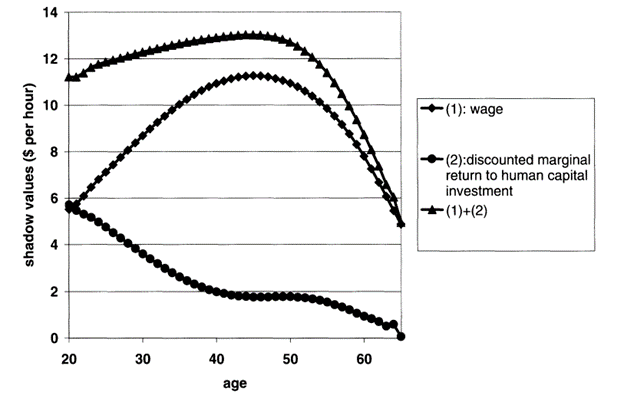
\includegraphics[width=6in]{\FigDir/Figure7}}
  \caption{AGE SHADOW WAGE PROFILES}
  \label{fig:AgeShadow}
\end{figure}

        \hypertarget{TempIncrease}{}
\begin{figure}[tbp]
  \centerline{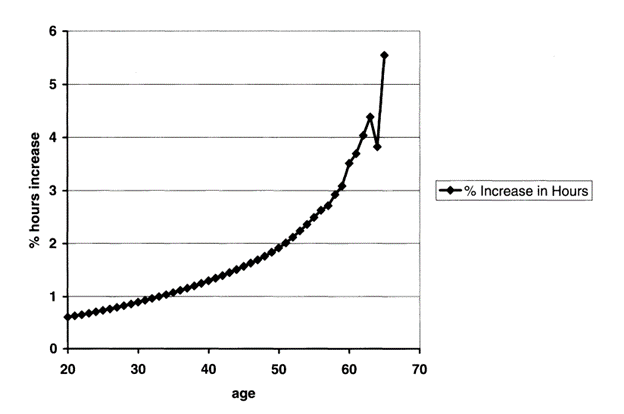
\includegraphics[width=6in]{\FigDir/Figure8}}
  \caption{PERCENT INCREASE IN HOURS DUE TO TEMPORARY 2\% INCREASE IN WAGES}
  \label{fig:TempIncrease}
\end{figure}

         Finally, we consider the implications of our model for the elasticity of hours with respect to wages. In Figure \ref{fig:TempIncrease}, we plot the change in age $t$ hours due to a 2\% temporary increase in the age t wage payment, holding human capital fixed. This experiment can be interpreted as a temporary increase in rental rate for human capital by 2\%. For a person at age 20, it only increases hours by around 0.6\%. But the elasticity of hours with respect to the current wage becomes larger with age. At around age 60, hours increase by more than 4\%. That is, with age, hours become more responsive to wage changes. This supports the claim that when young, because of the high human capital investment returns, labor supply is insensitive to the wage change. But when old, since the human capital effect is relatively insignificant, hours respond much more to wage changes. \cite{Shaw1989-jb} noted that the human capital model implies this pattern.
\end{document}
